\documentclass{assignment}
\usepackage{hyperref}
\usepackage{caption}
\usepackage{listings}
\usepackage[utf8]{inputenc}
\usepackage[T1]{fontenc}
\usepackage{babel}
\usepackage{graphicx}
\usepackage{listings}
\usepackage{assignment}
\usepackage{tikz}
\lstset{
    language=C++,
    basicstyle=\small,       % font size
    breaklines=true,         % line wrap
    postbreak=\raisebox{0ex}[0ex][0ex]{\ensuremath{\color{red}\hookrightarrow\space}},        % arrow on wrapped lines
    literate={\ \ }{{\ }}1   % adjust tab size
}

\newcommand*{\name}{Roberto Alvarado}
\newcommand*{\id}{00206411}
\newcommand*{\course}{Computer Networks}
\newcommand*{\assignment}{Homework 3}

\begin{document}
\assignmentTitle{\name}{\id}{logo.png}{\course}{\assignment}
\begin{ex}
   Read the following Wireshark tutorial, and use it to capture traffic from the following scenarios.
Use screenshots to show your results.
\begin{itemize}
  
\item Run 10 traceroute commands against google.com
\item Watch a video from youtube.com. Capture the TCP handshake, and the congestion window. 
\end{itemize}
\end{ex}
\begin{itemize}
  \item Results of 10 traceroute commands
    \begin{figure}[h]
      \begin{center}
        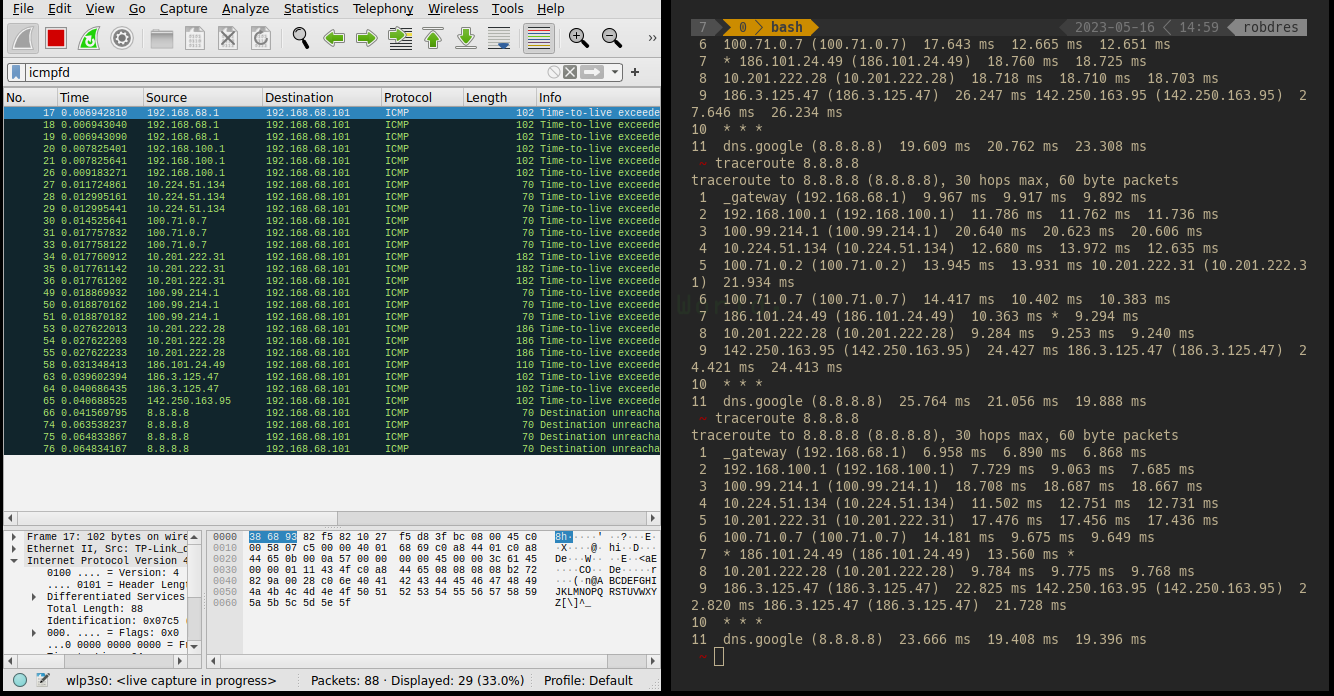
\includegraphics[width=0.45\textwidth]{1001.png}
      \end{center}
      \label{fig:}
    \end{figure}
    \begin{figure}[h]
      \begin{center}
        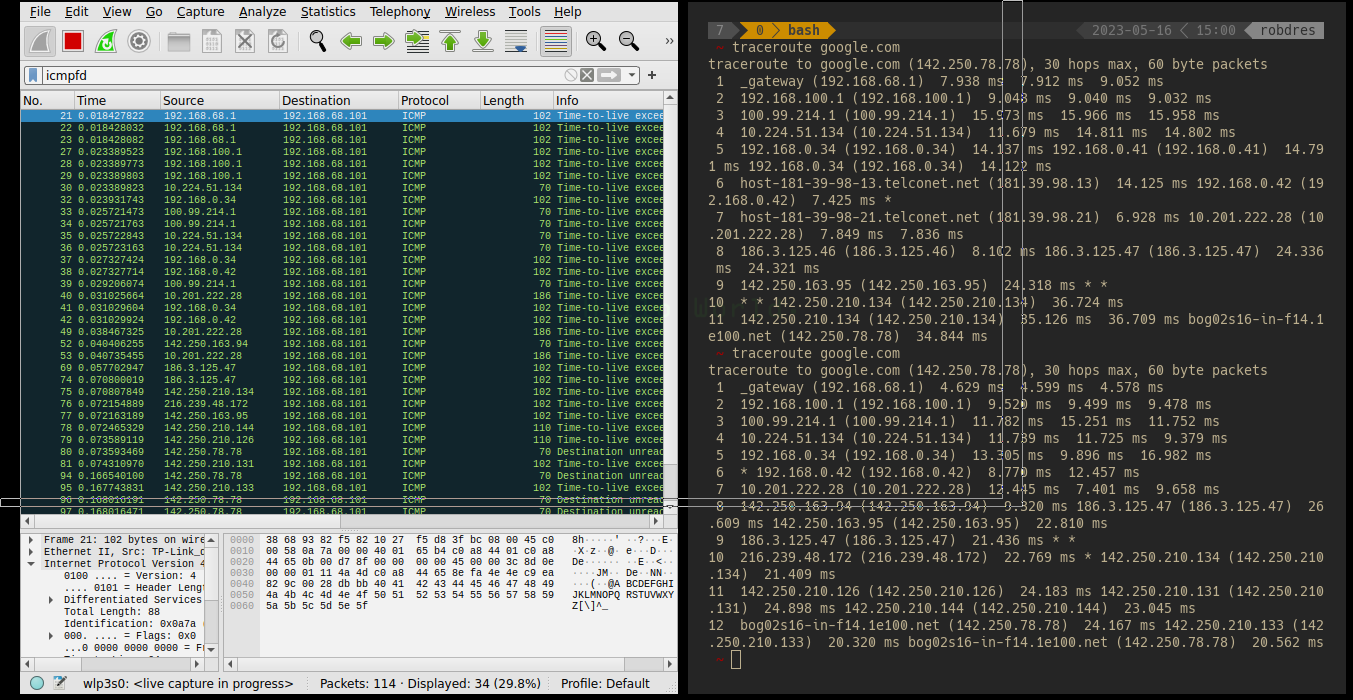
\includegraphics[width=0.45\textwidth]{1002.png}
      \end{center}
      \label{fig:}
    \end{figure}
    \newpage
    \begin{figure}[h]
      \begin{center}
        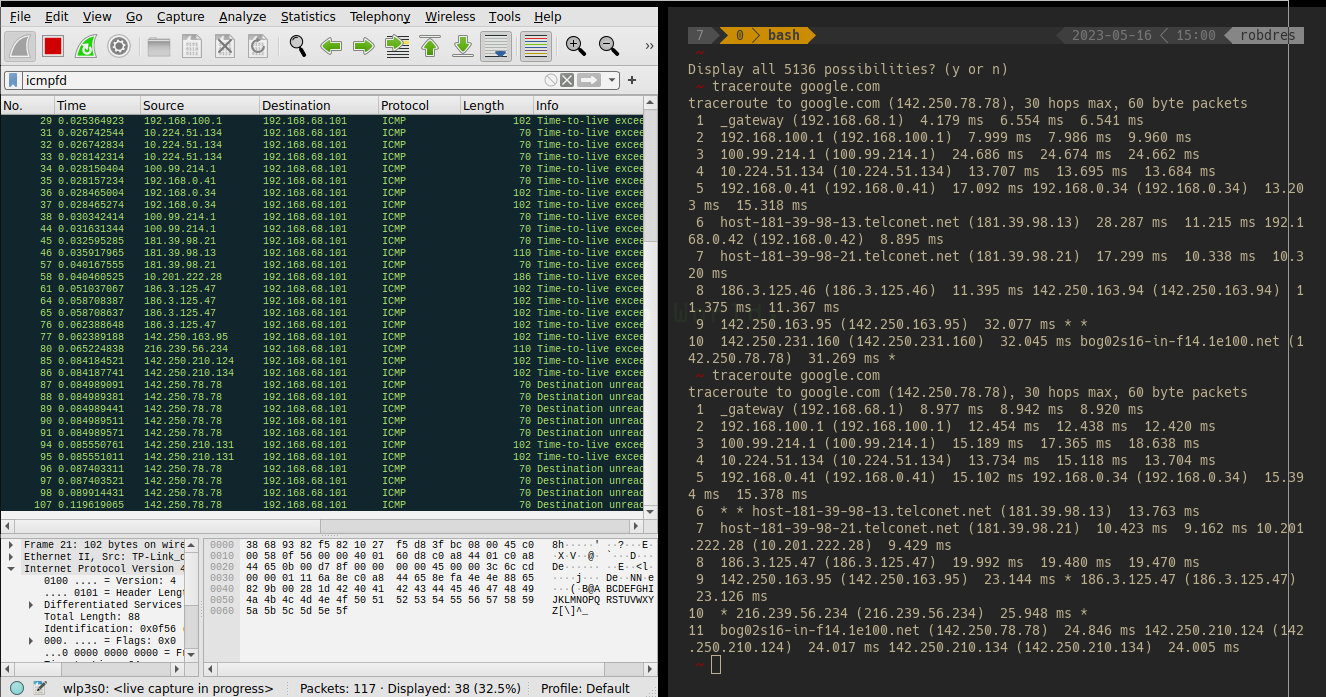
\includegraphics[width=0.45\textwidth]{1003.png}
      \end{center}
      \label{fig:}
    \end{figure}
    \begin{figure}[h]
      \begin{center}
        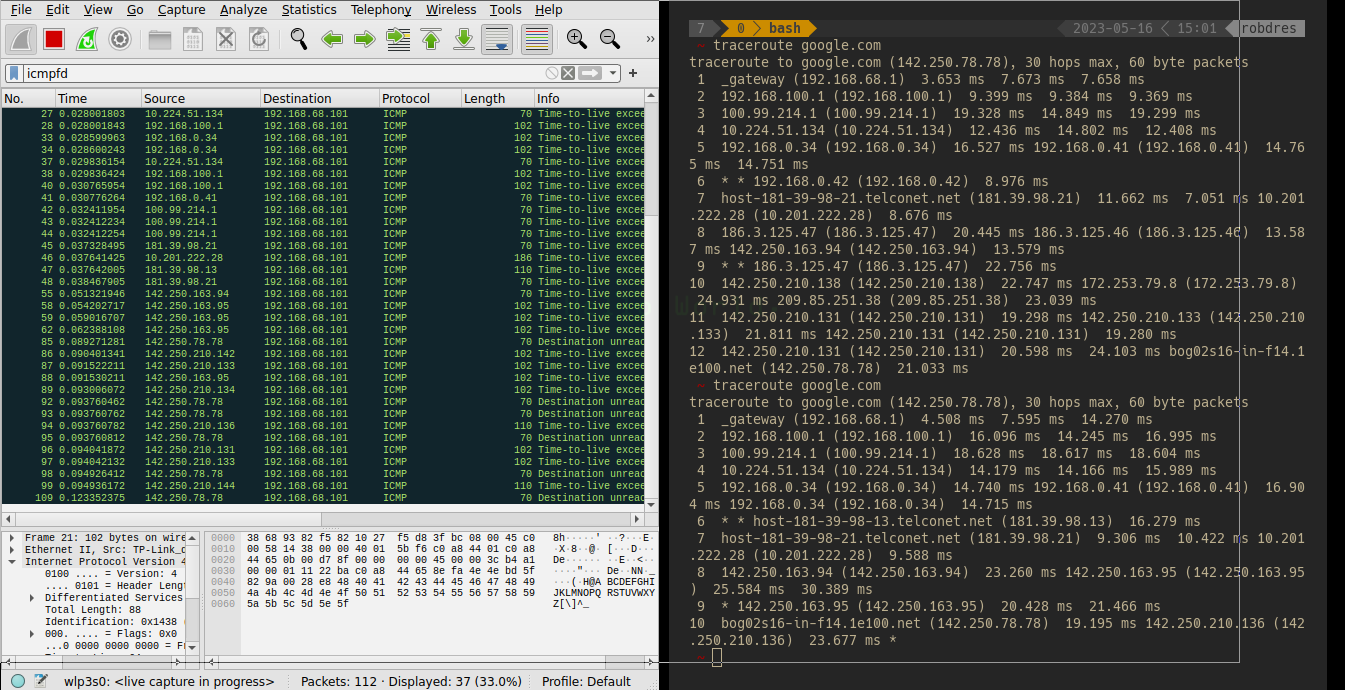
\includegraphics[width=0.45\textwidth]{1004.png}
      \end{center}
      \label{fig:}
    \end{figure}
    \begin{figure}[h]
      \begin{center}
        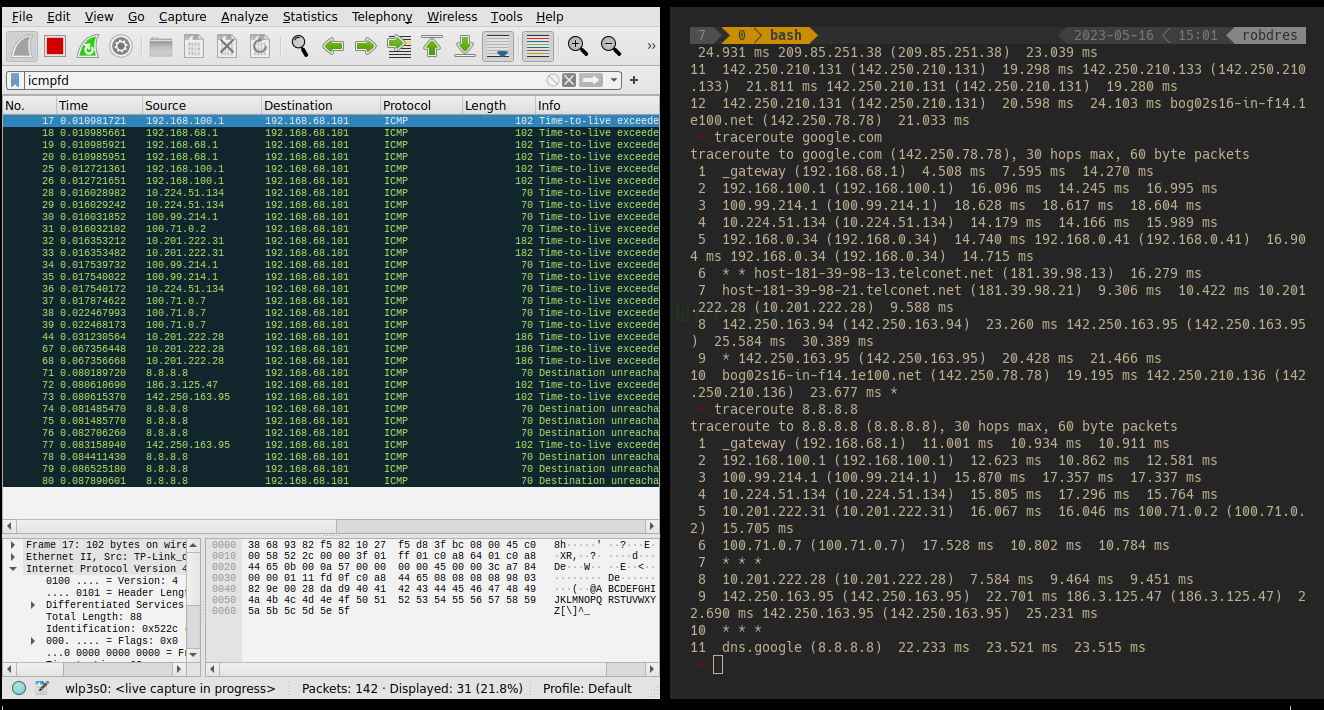
\includegraphics[width=0.45\textwidth]{1005.png}
      \end{center}
      \label{fig:}
    \end{figure}
    \newpage
    \begin{figure}[h]
      \begin{center}
        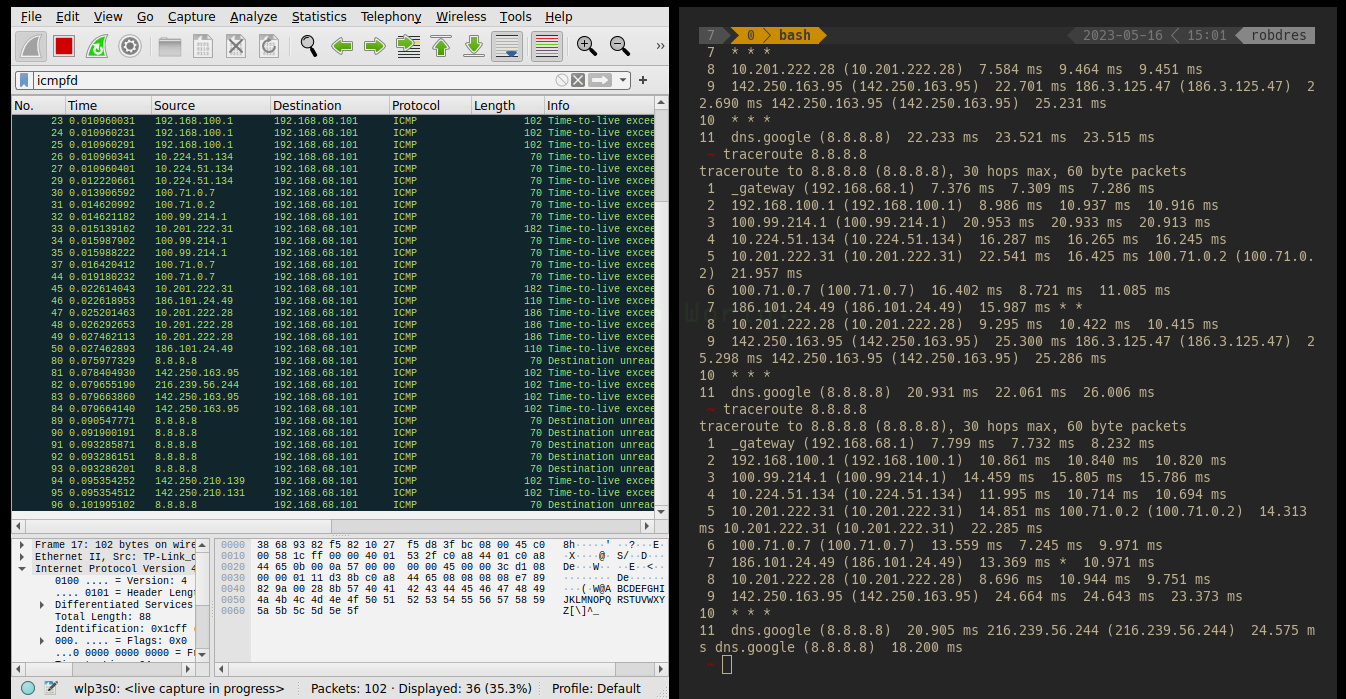
\includegraphics[width=0.45\textwidth]{1006.png}
      \end{center}
      \label{fig:}
    \end{figure}
    \begin{figure}[h]
      \begin{center}
        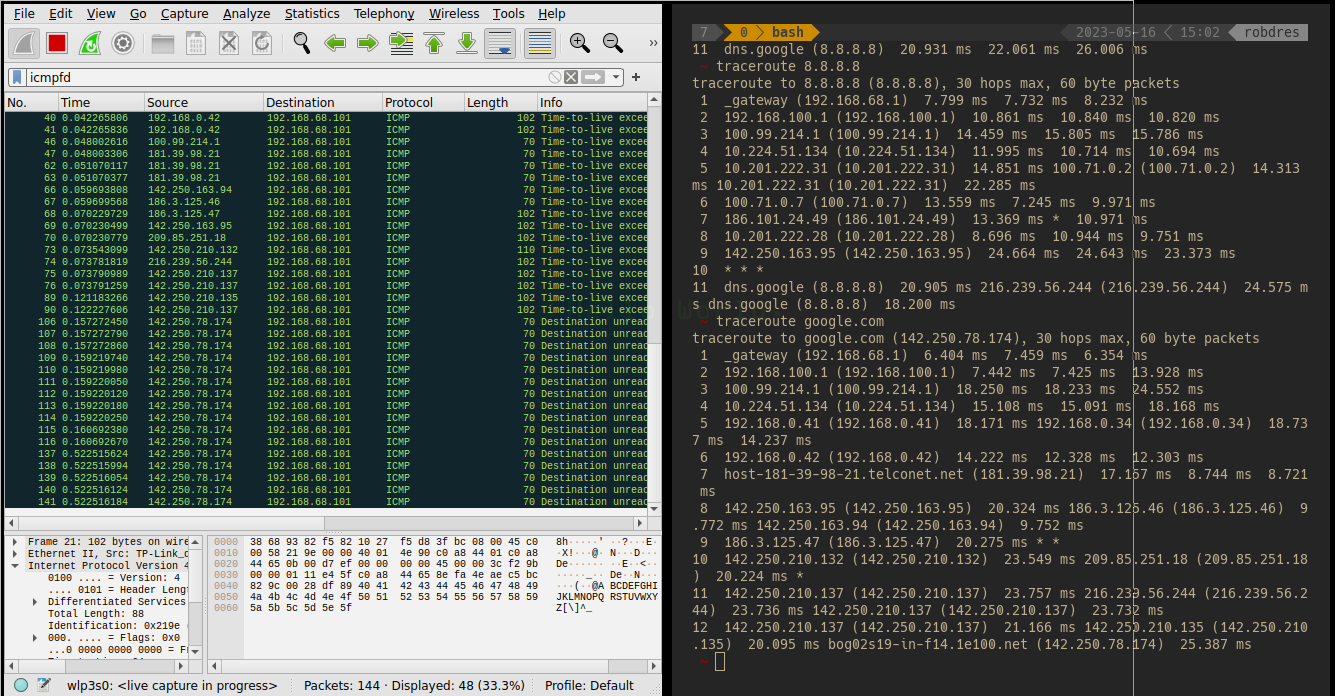
\includegraphics[width=0.45\textwidth]{1007.png}
      \end{center}
      \label{fig:}
    \end{figure}
    \newpage
    \begin{figure}[h]
      \begin{center}
        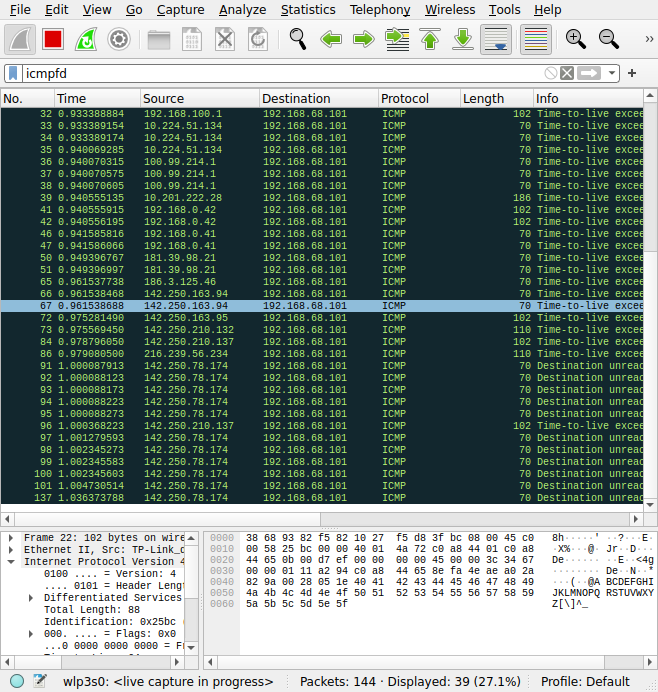
\includegraphics[width=0.35\textwidth]{1008.png}
      \end{center}
      \label{fig:}
    \end{figure}
    \begin{figure}[h]
      \begin{center}
        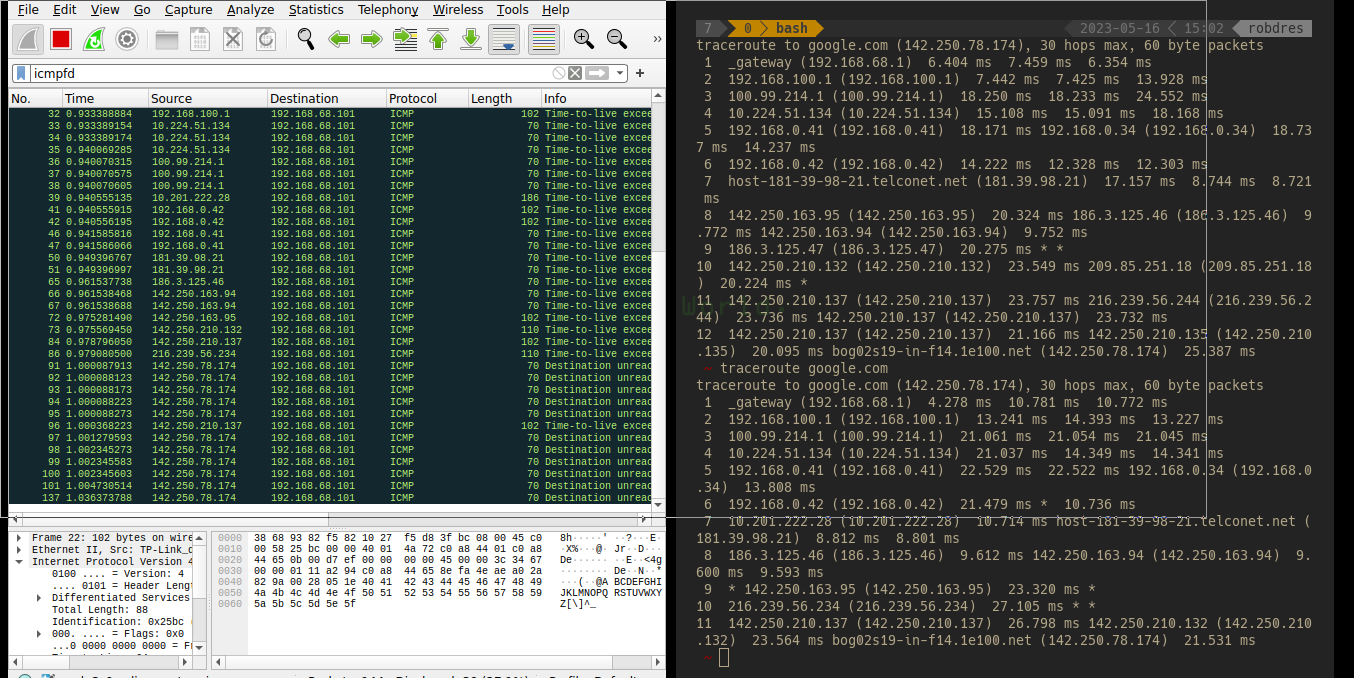
\includegraphics[width=0.35\textwidth]{1009.png}
      \end{center}
      \label{fig:}
    \end{figure}

    \begin{figure}[h]
      \begin{center}
        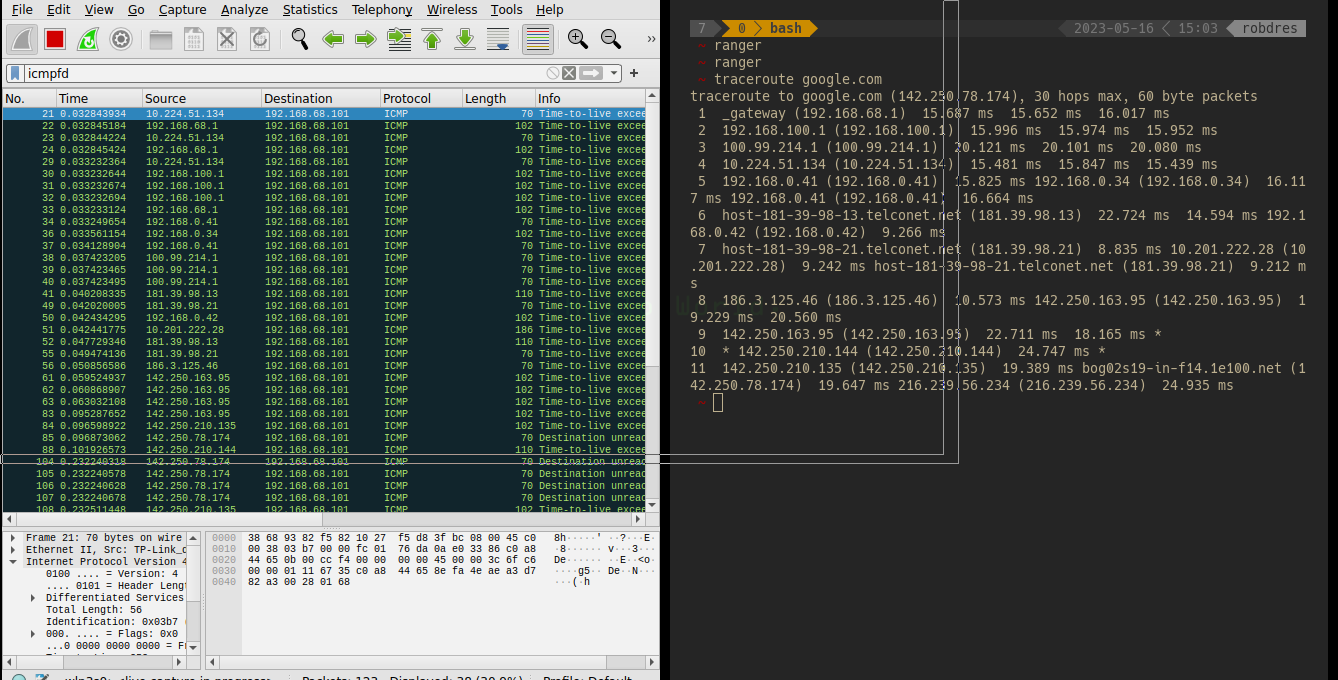
\includegraphics[width=0.35\textwidth]{1010.png}
      \end{center}
      \label{fig:}
    \end{figure}
\newpage
  \item Now first the handshake
    \begin{figure}[h]
      \begin{center}
        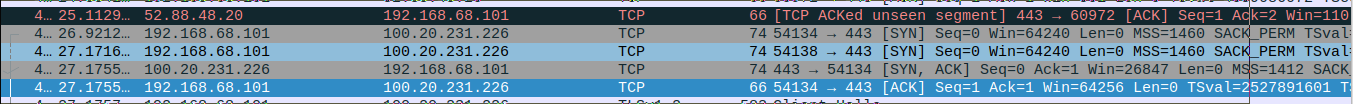
\includegraphics[width=0.95\textwidth]{100.png}
      \end{center}
      \label{fig:}
    \end{figure}
    And now the results 
    \begin{figure}[h]
      \begin{center}
        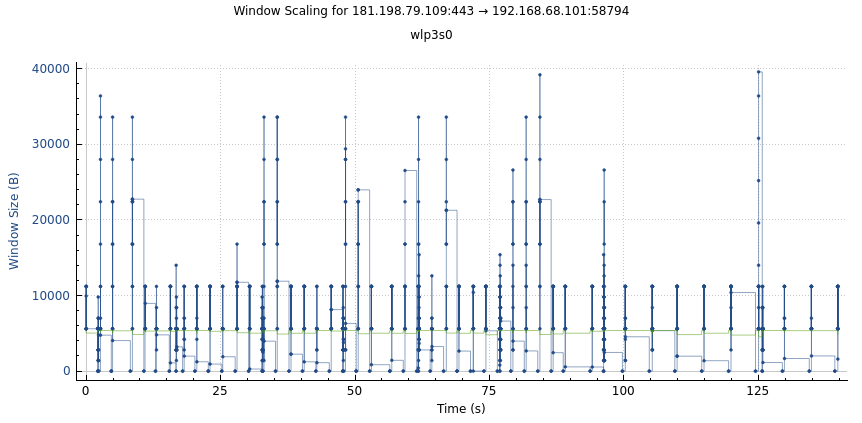
\includegraphics[width=0.75\textwidth]{CongestionWIndow.png}
      \end{center}
      \label{fig:}
    \end{figure}
    \begin{figure}[h]
      \begin{center}
        \includegraphics[width=0.75\textwidth]{CongestionStream1.png}
      \end{center}
      \label{fig:}
    \end{figure}

\end{itemize}


\newpage
\begin{ex}
Use Dijkstra's to get the routing tables for nodes A, B and E.
\end{ex}
\begin{figure}[h]
\begin{center}
  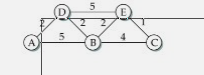
\includegraphics[scale=0.98]{1.png}
\end{center}
\label{fig:fig}
\end{figure}
\textit{ Sol. }

\begin{lstlisting}[language=Python]
  
from queue import PriorityQueue
class Graph:
    def __init__(self, num_of_vertices):
        self.v = num_of_vertices
        self.edges = [[-1 for i in range(num_of_vertices)] for j in range(num_of_vertices)]
        self.visited = []
    def add_edge(self, u, v, weight):
        self.edges[u][v] = weight
        self.edges[v][u] = weight

def dijkstra(graph, start_vertex):
    D = {v:float('inf') for v in range(graph.v)}
    D[start_vertex] = 0

    pq = PriorityQueue()
    pq.put((0, start_vertex))

    while not pq.empty():
        (dist, current_vertex) = pq.get()
        graph.visited.append(current_vertex)

        for neighbor in range(graph.v):
            if graph.edges[current_vertex][neighbor] != -1:
                distance = graph.edges[current_vertex][neighbor]
                if neighbor not in graph.visited:
                    old_cost = D[neighbor]
                    new_cost = D[current_vertex] + distance
                    if new_cost < old_cost:
                        pq.put((new_cost, neighbor))
                        D[neighbor] = new_cost
    return D

g = Graph(5)
g.add_edge(0,1,5)
g.add_edge(0,3,2)
g.add_edge(1,3,2)
g.add_edge(1,4,2)
g.add_edge(1,2,4)
g.add_edge(2,4,1)
g.add_edge(3,4,5)

print(dijkstra(g,0))
\end{lstlisting}

El resultado es 
\begin{lstlisting}
  {0: 0, 1: 4, 2: 7, 3: 2, 4: 6}
\end{lstlisting}
Entonces routing tables

\begin{minipage}{0.4\textwidth}
  \centering
  
    \begin{tabular}[c]{l|l}
      \hline
      \multicolumn{1}{c|}{\textbf{Node}} & 
      \multicolumn{1}{c}{\textbf{Next}} \\
      \hline
      B & D\\
      C & D\\
      D & D\\
      E & D\\
      \hline
    \end{tabular}

    \begin{tabular}[c]{l|l}
      \hline
      \multicolumn{1}{c|}{\textbf{Node}} & 
      \multicolumn{1}{c}{\textbf{Next}} \\
      \hline
      A & D\\
      C & E\\
      D & D\\
      E & E\\
      \hline
    \end{tabular}

    \begin{tabular}[c]{l|l}
      \hline
      \multicolumn{1}{c|}{\textbf{Node}} & 
      \multicolumn{1}{c}{\textbf{Next}} \\
      \hline
      A & E\\
      B & E\\
      D & E\\
      E & E\\
      \hline
    \end{tabular}

\end{minipage}
\begin{minipage}{0.4\textwidth}
  \centering
    \begin{tabular}[c]{l|l}
      \hline
      \multicolumn{1}{c|}{\textbf{Node}} & 
      \multicolumn{1}{c}{\textbf{Next}} \\
      \hline
      A & A\\
      B & B\\
      C & B\\
      E & B\\
      \hline
    \end{tabular}

    \begin{tabular}[c]{l|l}
      \hline
      \multicolumn{1}{c|}{\textbf{Node}} & 
      \multicolumn{1}{c}{\textbf{Next}} \\
      \hline
      A & B\\
      B & B\\
      C & C\\
      D & B\\
      \hline
    \end{tabular}
\end{minipage}
\newpage
\begin{ex}
Suppose a host wants to establish the reliability of a link by sending packets and measuring
the percentage that are received; routers, for example, do this. Explain the difficulty of doing
this over a TCP connection.
\end{ex}
\textit{ Sol. }
There is one main reason why using TCP, could be a problem. The way that it
manages lost packages or broken packages, as if a package in this protocol is
lost, then it will be retransmitted, but the sending host will only receive the
response from the destination host, it will not know if the package was
retransmitted, if we could add a tag to the package if it was retransmitted.

So at the end if we want to manage this analysis using TCP, as we could be
receiving ACK, without knowing the loss, then we could add maybe a TIME tag so
that we manage it
\newpage
\begin{ex}
Consider a simple congestion control algorithm that uses linear increase and multiplicative
decrease (no slow start). Assume the congestion window size is in units of packets rather than
bytes, and it is one packet initially.
\begin{itemize}
\item Give a detailed sketch of this algorithm.
\item Assume the delay is latency only, and that when a group of packets is sent, only a single
ACK is returned.
\item Plot the congestion window as a function of RTT for the situation in which the following
packets are lost: 9, 25, 30, 38 and 50. For simplicity, assume a perfect timeout mechanism
that detects a lost packet exactly 1 RTT after it is transmitted. 
\end{itemize}
  
\end{ex}
\textit{ Sol. }

\begin{itemize}

\item The idea of the algorithm is 
  \begin{lstlisting}[]
  [IF ACK] cwnd <- cwnd+a
  [IF TIMEOUT] cwnd <- cwnd/b
  \end{lstlisting} 
  Parameters have to be defined has to be define, let $a=1, b =2$
  \item
In this case  we could use an example on how it would increases, and using the case of the last example
    \begin{figure}[h]
      \begin{center}
        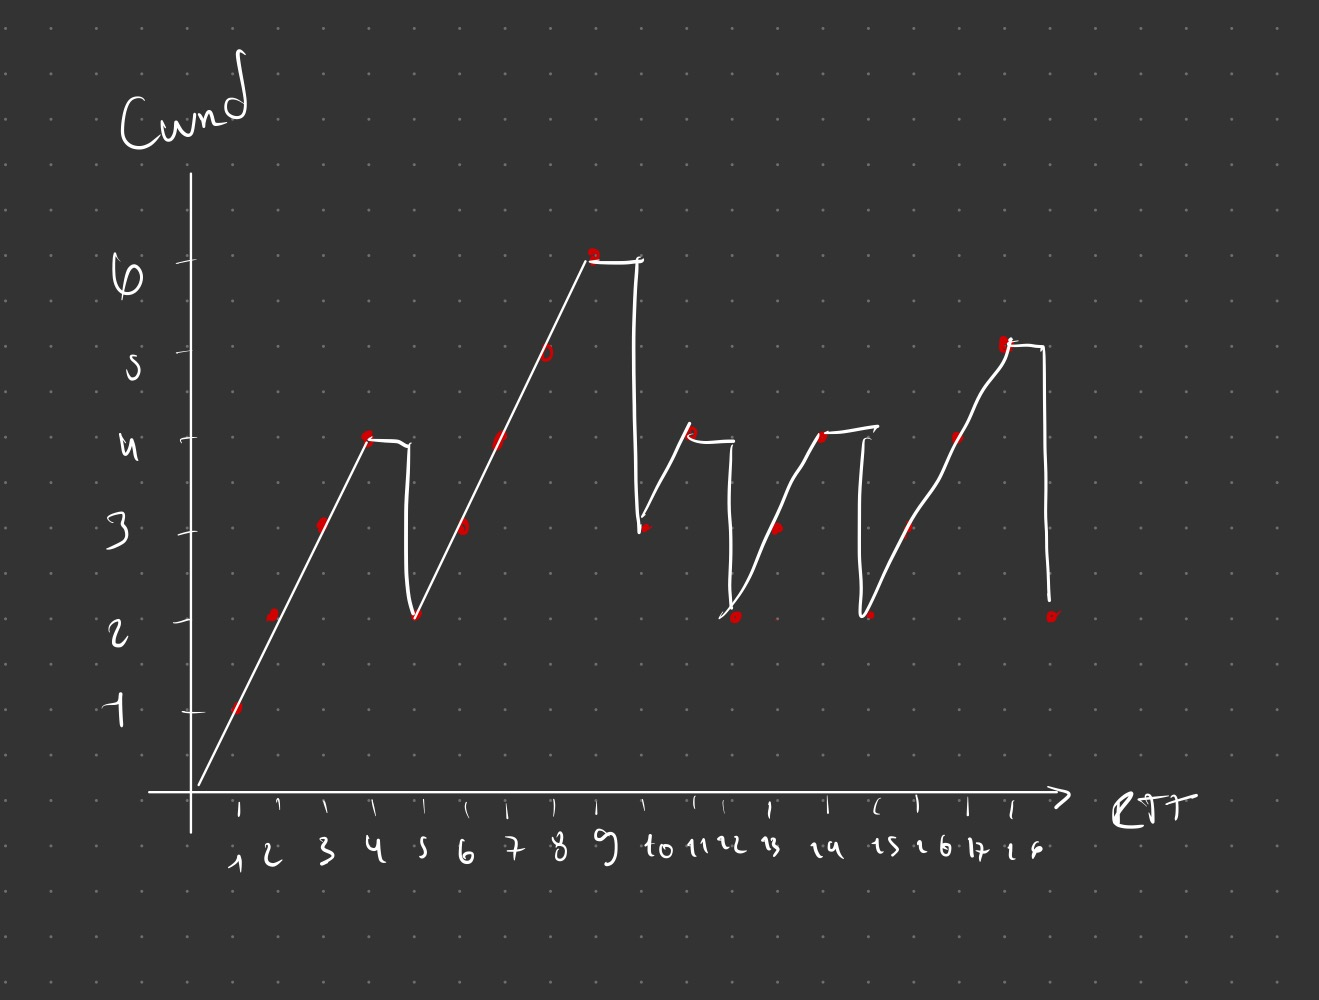
\includegraphics[width=0.7\textwidth]{public.jpeg}
      \end{center}
      \caption{}
      \label{fig:}
    \end{figure}
\item 
  \begin{table}[h]
    \caption{}
    \label{tab:}
    \begin{center}
      \begin{tabular}[c]{c|c|c}
        \hline
        \multicolumn{1}{c|}{\textbf{RTT STEP}} & 
        \multicolumn{1}{c|}{\textbf{Last Package Sent}} & 
        \multicolumn{1}{c}{\textbf{\# packages sent}} \\
        \hline
        1  & 1 & 1\\
        1  & 3 & 2\\
        2  & 6 & 3\\
        3  & 10 & 4\\
        4  & 9-10 & 2\\
        5  & 13 & 3 \\
        6  & 15 & 4\\
        7  & 22 & 5\\
        8  & 28 & 6\\
        9  & 25-27 & 3\\
        10 & 32 & 4\\
        11 & 30-31 & 2\\
        12 & 34 & 3 \\
        13 & 38 & 4 \\
        14 & 38-39 & 2 \\
        15 & 42 & 3 \\
        16 & 46 & 4 \\
        17 & 51 & 5 \\
        18 & 50-51 & 2 \\
        \hline

      \end{tabular}
    \end{center}
  \end{table}
  \\
    
  
\end{itemize}
\end{document}
